\documentclass[9pt]{beamer}
\usetheme{cmepda}

\usepackage[utf8]{inputenc}
\usepackage[T1]{fontenc}

\graphicspath{{figures/}} 


\title{Advanced python features - part II}
\subtitle{Computing Methods for Experimental Physics and Data Analysis}
\date{Compiled on \today}
\author{A. Manfreda}
\institute[INFN]{INFN--Pisa}
\email{alberto.manfreda@pi.infn.it}


\begin{document}


\titleframe


\begin{frame}
  \frametitle{Functions inside functions}
  \begin{itemize}
    \item Function in python are \alert{first class object}
    \item The name is a bit misleading, but what actually means is that functions
          can be passed as argument to other functions and returned as result from
          other functions
    \item This shouldn't surprise you much: functions are objects of a
          '\emph{function}' class, so they behave like any other vairable in
          Python
    \item Another thing you can (and sometimes want to) do is \emph{defining} a
          function inside another.
    \item Let's see how it works
  \end{itemize}
  
\end{frame}


\begin{frame}
  \frametitle{Functions inside functions}
  \begin{Verbatim}[label=\makebox{\url{https://github.com/lucabaldini/cmepda/tree/master/slides/latex/snippets/inner\_outer.py}},commandchars=\\\{\}]
\PY{k}{def} \PY{n+nf}{outer}\PY{p}{(}\PY{p}{)}\PY{p}{:}   
    \PY{k}{def} \PY{n+nf}{inner}\PY{p}{(}\PY{p}{)}\PY{p}{:} \PY{c+c1}{\PYZsh{} Defining the inner function inside the outer function}
        \PY{k}{print}\PY{p}{(}\PY{l+s+s1}{\PYZsq{}}\PY{l+s+s1}{Inner function}\PY{l+s+s1}{\PYZsq{}}\PY{p}{)}
        \PY{k}{return} \PY{c+c1}{\PYZsh{} End of the inner function}
    \PY{k}{return} \PY{n}{inner} \PY{c+c1}{\PYZsh{} Inner is the output of outer}
    
\PY{n}{my\PYZus{}func} \PY{o}{=} \PY{n}{outer}\PY{p}{(}\PY{p}{)} \PY{c+c1}{\PYZsh{} my\PYZus{}func is now referncing \PYZsq{}inner\PYZsq{}}
\PY{k}{print}\PY{p}{(}\PY{n}{my\PYZus{}func}\PY{o}{.}\PY{n+nv+vm}{\PYZus{}\PYZus{}name\PYZus{}\PYZus{}}\PY{p}{)}
\PY{n}{my\PYZus{}func}\PY{p}{(}\PY{p}{)} \PY{c+c1}{\PYZsh{} Calling my\PYZus{}func is equal to calling \PYZsq{}inner\PYZsq{}}

\PY{k}{def} \PY{n+nf}{outer2}\PY{p}{(}\PY{p}{)}\PY{p}{:}
    \PY{n}{some\PYZus{}string} \PY{o}{=} \PY{l+s+s1}{\PYZsq{}}\PY{l+s+s1}{Hello!}\PY{l+s+s1}{\PYZsq{}}
    \PY{k}{def} \PY{n+nf}{inner}\PY{p}{(}\PY{p}{)}\PY{p}{:}
        \PY{c+c1}{\PYZsh{} We have access to the variables in the outer function!}
        \PY{k}{print}\PY{p}{(}\PY{n}{some\PYZus{}string}\PY{p}{)}
    \PY{k}{return} \PY{n}{inner}
    
\PY{n}{my\PYZus{}other\PYZus{}func} \PY{o}{=} \PY{n}{outer2}\PY{p}{(}\PY{p}{)}
\PY{n}{my\PYZus{}other\PYZus{}func}\PY{p}{(}\PY{p}{)}

[Output]
inner
Inner function
Hello!
\end{Verbatim}
\end{frame}


\begin{frame}
  \frametitle{Colusers and free variables}
  \begin{itemize}
    \item When a function is created inside another function it has access to the local variables
          of the outer function, even after its scope ended
    \item This is techincally possible because those varibales are kept in a special
          space of memory, the \alert{closure} of the inner function
    \item Such variables are called \alert{free variables}
    \item Note: if you \emph{assign} to a free variable in the inner function, 
          by default a new, local variable is created instead!
    \item To avoid this you have to explictly declare that you want to access the variable in
          the closure using the \alert{nonlocal} keyword
    \item Remember: \emph{'Explicit is better then implicit'}
  \end{itemize}
  
\end{frame}


\begin{frame}
  \frametitle{Free variables - a mistake to avoid}
  \begin{Verbatim}[label=\makebox{\url{https://github.com/lucabaldini/cmepda/tree/master/slides/latex/snippets/closure\_wrong.py}},commandchars=\\\{\}]
\PY{k}{def} \PY{n+nf}{running\PYZus{}average}\PY{p}{(}\PY{p}{)}\PY{p}{:}
    \PY{n}{total\PYZus{}count} \PY{o}{=} \PY{l+m+mi}{0}
    \PY{n}{num\PYZus{}elements} \PY{o}{=} \PY{l+m+mi}{0}
    \PY{k}{def} \PY{n+nf}{accumulator}\PY{p}{(}\PY{n}{value}\PY{p}{)}\PY{p}{:}
        \PY{n}{total\PYZus{}count} \PY{o}{+}\PY{o}{=} \PY{n}{value} \PY{c+c1}{\PYZsh{} Doesn\PYZsq{}t work! total\PYZus{}count is reassigned!}
        \PY{n}{num\PYZus{}elements} \PY{o}{+}\PY{o}{=} \PY{l+m+mi}{1} \PY{c+c1}{\PYZsh{} Doesn\PYZsq{}t work! total\PYZus{}count is reassigned!}
        \PY{k}{return} \PY{n}{total\PYZus{}count}\PY{o}{/}\PY{n}{num\PYZus{}elements}
    \PY{k}{return} \PY{n}{accumulator}
    
\PY{n}{run\PYZus{}avg} \PY{o}{=} \PY{n}{running\PYZus{}average}\PY{p}{(}\PY{p}{)}
\PY{k}{print}\PY{p}{(}\PY{n}{run\PYZus{}avg}\PY{p}{(}\PY{l+m+mf}{1.}\PY{p}{)}\PY{p}{)}
\PY{k}{print}\PY{p}{(}\PY{n}{run\PYZus{}avg}\PY{p}{(}\PY{l+m+mf}{5.}\PY{p}{)}\PY{p}{)}
\PY{k}{print}\PY{p}{(}\PY{n}{run\PYZus{}avg}\PY{p}{(}\PY{l+m+mf}{2.5}\PY{p}{)}\PY{p}{)}

[Output]
Traceback (most recent call last):
  File "snippets/closure_wrong.py", line 11, in <module>
    print(run_avg(1.))
  File "snippets/closure_wrong.py", line 5, in accumulator
    total_count += value # Doesn't work! total_count is reassigned!
UnboundLocalError: local variable 'total_count' referenced before assignment
\end{Verbatim}
\end{frame}


\begin{frame}
  \frametitle{Free variables - the correct way}
  \begin{Verbatim}[label=\makebox{\url{https://github.com/lucabaldini/cmepda/tree/master/slides/latex/snippets/closure\_right.py}},commandchars=\\\{\}]
\PY{k}{def} \PY{n+nf}{running\PYZus{}average}\PY{p}{(}\PY{p}{)}\PY{p}{:}
    \PY{n}{total\PYZus{}count} \PY{o}{=} \PY{l+m+mi}{0}
    \PY{n}{num\PYZus{}elements} \PY{o}{=} \PY{l+m+mi}{0}
    \PY{k}{def} \PY{n+nf}{accumulator}\PY{p}{(}\PY{n}{value}\PY{p}{)}\PY{p}{:}
        \PY{c+c1}{\PYZsh{} We declare the relevant variables as nonlocal}
        \PY{n}{nonlocal} \PY{n}{total\PYZus{}count}\PY{p}{,} \PY{n}{num\PYZus{}elements}
        \PY{c+c1}{\PYZsh{} Now we can assign to them \PYZhy{} the variables in the closure will be}
        \PY{c+c1}{\PYZsh{} modified, as we want!}
        \PY{n}{total\PYZus{}count} \PY{o}{+}\PY{o}{=} \PY{n}{value}
        \PY{n}{num\PYZus{}elements} \PY{o}{+}\PY{o}{=} \PY{l+m+mi}{1}
        \PY{k}{return} \PY{n}{total\PYZus{}count}\PY{o}{/}\PY{n}{num\PYZus{}elements}
    \PY{k}{return} \PY{n}{accumulator}
    
\PY{n}{run\PYZus{}avg} \PY{o}{=} \PY{n}{running\PYZus{}average}\PY{p}{(}\PY{p}{)}
\PY{k}{print}\PY{p}{(}\PY{n}{run\PYZus{}avg}\PY{p}{(}\PY{l+m+mf}{1.}\PY{p}{)}\PY{p}{)}
\PY{k}{print}\PY{p}{(}\PY{n}{run\PYZus{}avg}\PY{p}{(}\PY{l+m+mf}{5.}\PY{p}{)}\PY{p}{)}
\PY{k}{print}\PY{p}{(}\PY{n}{run\PYZus{}avg}\PY{p}{(}\PY{l+m+mf}{2.5}\PY{p}{)}\PY{p}{)}

[Output]
1.0
3.0
2.8333333333333335
\end{Verbatim}
\end{frame}


\begin{frame}
  \frametitle{Wrapping functions}
  \begin{itemize}
    \item The typical use of defining a function inside a function is to create
          a \alert{wrapper}
    \item A wrapper is a function that calls another one adding a layer
          of functionalities in between - for example it may do some pre-process
          of the input, or change the output in some way, or measure the 
          execution time or whatever we want
    \item The techinque for creating a wrapper fucntion in Python is:
    \begin{itemize}
       \item Pass the function that we want to wrap as argument of the outer
             function
       \item Inside the outer function we define an inner function, which is the
             actual wrapper
       \item The wrapper calls the wrapped function and adds its functionalities,
             before and/or after the call. It may return the same output or a 
             manipulated one.
       \item Then from the outer fucntion we return the wrapper
    \end{itemize}
  \end{itemize}
  
\end{frame}


\begin{frame}
  \frametitle{Wrapper}
  \begin{Verbatim}[label=\makebox{\url{https://github.com/lucabaldini/cmepda/tree/master/slides/latex/snippets/wrapper.py}},commandchars=\\\{\}]
\PY{k}{def} \PY{n+nf}{some\PYZus{}function}\PY{p}{(}\PY{n}{a}\PY{p}{,} \PY{n}{b}\PY{p}{)}\PY{p}{:}
    \PY{k}{print}\PY{p}{(}\PY{l+s+s1}{\PYZsq{}}\PY{l+s+s1}{Executing \PYZob{}\PYZcb{} x \PYZob{}\PYZcb{}}\PY{l+s+s1}{\PYZsq{}}\PY{o}{.}\PY{n}{format}\PY{p}{(}\PY{n}{a}\PY{p}{,} \PY{n}{b}\PY{p}{)}\PY{p}{)}
    \PY{k}{return} \PY{n}{a} \PY{o}{*} \PY{n}{b}
    
\PY{k}{def} \PY{n+nf}{add\PYZus{}n\PYZus{}wrapper}\PY{p}{(}\PY{n}{func}\PY{p}{,} \PY{n}{n}\PY{p}{)}\PY{p}{:} \PY{c+c1}{\PYZsh{} We take the wrapped function as argument}
    \PY{l+s+sd}{\PYZdq{}\PYZdq{}\PYZdq{} This wrapper adds n to the result of the wrapped function\PYZdq{}\PYZdq{}\PYZdq{}}
    
    \PY{k}{def} \PY{n+nf}{wrapper}\PY{p}{(}\PY{o}{*}\PY{n}{args}\PY{p}{,} \PY{o}{*}\PY{o}{*}\PY{n}{kwargs}\PY{p}{)}\PY{p}{:} 
       \PY{l+s+sd}{\PYZdq{}\PYZdq{}\PYZdq{}We passs the arguments as *arg, **kwargs, because this is the most}
\PY{l+s+sd}{       general form in Python: we can collect any comination of arguments like}
\PY{l+s+sd}{       that. Note that we have access to both \PYZsq{}func\PYZsq{} and \PYZsq{}n\PYZsq{}, as they are stored}
\PY{l+s+sd}{       in the closure of \PYZsq{}wrapper\PYZsq{}\PYZdq{}\PYZdq{}\PYZdq{}}
       \PY{n}{result} \PY{o}{=} \PY{n}{func}\PY{p}{(}\PY{o}{*}\PY{n}{args}\PY{p}{,} \PY{o}{*}\PY{o}{*}\PY{n}{kwargs}\PY{p}{)} \PY{c+c1}{\PYZsh{} Pass the arguments to the wrapped fucntion}
       \PY{k}{print}\PY{p}{(}\PY{l+s+s1}{\PYZsq{}}\PY{l+s+s1}{Adding \PYZob{}\PYZcb{}}\PY{l+s+s1}{\PYZsq{}}\PY{o}{.}\PY{n}{format}\PY{p}{(}\PY{n}{n}\PY{p}{)}\PY{p}{)}
       \PY{k}{return} \PY{n}{result} \PY{o}{+} \PY{n}{n} \PY{c+c1}{\PYZsh{} Return a modified result in this case}
       
    \PY{k}{return} \PY{n}{wrapper} \PY{c+c1}{\PYZsh{} From add\PYZus{}n\PYZus{}wrapper we return the wrapper}

\PY{n}{function\PYZus{}plus\PYZus{}five} \PY{o}{=} \PY{n}{add\PYZus{}n\PYZus{}wrapper}\PY{p}{(}\PY{n}{some\PYZus{}function}\PY{p}{,} \PY{l+m+mi}{5}\PY{p}{)}
\PY{k}{print}\PY{p}{(}\PY{l+s+s1}{\PYZsq{}}\PY{l+s+s1}{Result = \PYZob{}\PYZcb{}}\PY{l+s+s1}{\PYZsq{}}\PY{o}{.}\PY{n}{format}\PY{p}{(}\PY{n}{function\PYZus{}plus\PYZus{}five}\PY{p}{(}\PY{l+m+mi}{2}\PY{p}{,} \PY{l+m+mi}{3}\PY{p}{)}\PY{p}{)}\PY{p}{)}

[Output]
Executing 2 x 3
Adding 5
Result = 11
\end{Verbatim}
\end{frame}


\begin{frame}
  \frametitle{Decorators}
  \begin{itemize}
    \item Often, when you wrap a function, you don't want to change
          it's name, so you reassign the wrapped funtion to its old name
    \item In fact, this techinque is so common that python introduced a special
          syntax for it: decorators
    \item A decorated function has simply the name of the wrapper added with
          a '@' on top of its declaration
  \end{itemize}
  
\end{frame}


\begin{frame}
  \frametitle{Decorators}
  \begin{Verbatim}[label=\makebox{\url{https://github.com/lucabaldini/cmepda/tree/master/slides/latex/snippets/decorator.py}},commandchars=\\\{\}]
\PY{k}{def} \PY{n+nf}{print\PYZus{}function\PYZus{}info}\PY{p}{(}\PY{n}{func}\PY{p}{)}\PY{p}{:}
    \PY{k}{def} \PY{n+nf}{wrapper}\PY{p}{(}\PY{o}{*}\PY{n}{args}\PY{p}{,} \PY{o}{*}\PY{o}{*}\PY{n}{kwargs}\PY{p}{)}\PY{p}{:}
        \PY{k}{print}\PY{p}{(}\PY{l+s+s1}{\PYZsq{}}\PY{l+s+s1}{Calling function }\PY{l+s+se}{\PYZbs{}\PYZsq{}}\PY{l+s+s1}{\PYZob{}\PYZcb{}}\PY{l+s+se}{\PYZbs{}\PYZsq{}}\PY{l+s+s1}{\PYZsq{}}\PY{o}{.}\PY{n}{format}\PY{p}{(}\PY{n}{func}\PY{o}{.}\PY{n+nv+vm}{\PYZus{}\PYZus{}name\PYZus{}\PYZus{}}\PY{p}{)}\PY{p}{)}
        \PY{k}{print}\PY{p}{(}\PY{l+s+s1}{\PYZsq{}}\PY{l+s+s1}{Positional arguments = \PYZob{}\PYZcb{}}\PY{l+s+s1}{\PYZsq{}}\PY{o}{.}\PY{n}{format}\PY{p}{(}\PY{n}{args}\PY{p}{)}\PY{p}{)}
        \PY{k}{print}\PY{p}{(}\PY{l+s+s1}{\PYZsq{}}\PY{l+s+s1}{Keyword arguments = \PYZob{}\PYZcb{}}\PY{l+s+s1}{\PYZsq{}}\PY{o}{.}\PY{n}{format}\PY{p}{(}\PY{n}{kwargs}\PY{p}{)}\PY{p}{)}
        \PY{k}{return} \PY{n}{func}\PY{p}{(}\PY{o}{*}\PY{n}{args}\PY{p}{,} \PY{o}{*}\PY{o}{*}\PY{n}{kwargs}\PY{p}{)}
    \PY{k}{return} \PY{n}{wrapper}

\PY{n+nd}{@print\PYZus{}function\PYZus{}info}
\PY{k}{def} \PY{n+nf}{some\PYZus{}function}\PY{p}{(}\PY{n}{a}\PY{p}{,} \PY{n}{b}\PY{p}{,} \PY{n}{c}\PY{o}{=}\PY{l+m+mi}{0}\PY{p}{)}\PY{p}{:}
    \PY{k}{return} \PY{n}{a} \PY{o}{*} \PY{n}{b} \PY{o}{+} \PY{n}{c}

\PY{c+c1}{\PYZsh{} This is equivalent to: some\PYZus{}function = print\PYZus{}function\PYZus{}info(some\PYZus{}function)}

\PY{k}{print}\PY{p}{(}\PY{n}{some\PYZus{}function}\PY{p}{(}\PY{l+m+mi}{1}\PY{p}{,} \PY{l+m+mi}{2}\PY{p}{,} \PY{n}{c}\PY{o}{=}\PY{l+m+mi}{7}\PY{p}{)}\PY{p}{)}
 \PY{c+c1}{\PYZsh{} Inspecting the function reveals that we are calling the wrapper}
\PY{k}{print}\PY{p}{(}\PY{l+s+s1}{\PYZsq{}}\PY{l+s+s1}{The name of the function is }\PY{l+s+se}{\PYZbs{}\PYZsq{}}\PY{l+s+s1}{\PYZob{}\PYZcb{}}\PY{l+s+se}{\PYZbs{}\PYZsq{}}\PY{l+s+s1}{\PYZsq{}}\PY{o}{.}\PY{n}{format}\PY{p}{(}\PY{n}{some\PYZus{}function}\PY{o}{.}\PY{n+nv+vm}{\PYZus{}\PYZus{}name\PYZus{}\PYZus{}}\PY{p}{)}\PY{p}{)}

[Output]
Calling function 'some_function'
Positional arguments = (1, 2)
Keyword arguments = {'c': 7}
9
The name of the function is 'wrapper'
\end{Verbatim}
\end{frame}


\begin{frame}
  \frametitle{A decorator to measure execution time}
  \begin{Verbatim}[label=\makebox{\url{https://github.com/lucabaldini/cmepda/tree/master/slides/latex/snippets/time\_measuring\_decor.py}},commandchars=\\\{\}]
\PY{k+kn}{import} \PY{n+nn}{time} 
\PY{k+kn}{from} \PY{n+nn}{functools} \PY{k+kn}{import} \PY{n}{wraps}

\PY{k}{def} \PY{n+nf}{clocked}\PY{p}{(}\PY{n}{func}\PY{p}{)}\PY{p}{:}
    \PY{l+s+sd}{\PYZdq{}\PYZdq{}\PYZdq{} We use functools.wraps to keep the original function name and docstring\PYZdq{}\PYZdq{}\PYZdq{}}
    \PY{n+nd}{@wraps}\PY{p}{(}\PY{n}{func}\PY{p}{)}
    \PY{k}{def} \PY{n+nf}{wrapper}\PY{p}{(}\PY{o}{*}\PY{n}{args}\PY{p}{,} \PY{o}{*}\PY{o}{*}\PY{n}{kwargs}\PY{p}{)}\PY{p}{:}
        \PY{n}{tstart} \PY{o}{=} \PY{n}{time}\PY{o}{.}\PY{n}{clock}\PY{p}{(}\PY{p}{)}
        \PY{n}{result} \PY{o}{=} \PY{n}{func}\PY{p}{(}\PY{o}{*}\PY{n}{args}\PY{p}{,} \PY{o}{*}\PY{o}{*}\PY{n}{kwargs}\PY{p}{)}
        \PY{n}{exec\PYZus{}time} \PY{o}{=} \PY{n}{time}\PY{o}{.}\PY{n}{clock}\PY{p}{(}\PY{p}{)} \PY{o}{\PYZhy{}} \PY{n}{tstart}
        \PY{k}{print}\PY{p}{(}\PY{l+s+s1}{\PYZsq{}}\PY{l+s+s1}{Function \PYZob{}\PYZcb{} executed in \PYZob{}\PYZcb{} s}\PY{l+s+s1}{\PYZsq{}}\PY{o}{.}\PY{n}{format}\PY{p}{(}\PY{n}{func}\PY{o}{.}\PY{n+nv+vm}{\PYZus{}\PYZus{}name\PYZus{}\PYZus{}}\PY{p}{,} \PY{n}{exec\PYZus{}time}\PY{p}{)}\PY{p}{)}
        \PY{k}{return} \PY{n}{result}
    \PY{k}{return} \PY{n}{wrapper}

\PY{n+nd}{@clocked}
\PY{k}{def} \PY{n+nf}{square\PYZus{}list}\PY{p}{(}\PY{n}{input\PYZus{}list}\PY{p}{)}\PY{p}{:}
    \PY{l+s+sd}{\PYZdq{}\PYZdq{}\PYZdq{} Return the square of a list\PYZdq{}\PYZdq{}\PYZdq{}}
    \PY{k}{return} \PY{p}{[}\PY{n}{item}\PY{o}{*}\PY{o}{*}\PY{l+m+mi}{2} \PY{k}{for} \PY{n}{item} \PY{o+ow}{in} \PY{n}{input\PYZus{}list}\PY{p}{]}

\PY{c+c1}{\PYZsh{} Make sure the function name and docstring look the same}
\PY{k}{print}\PY{p}{(}\PY{l+s+s1}{\PYZsq{}}\PY{l+s+se}{\PYZbs{}\PYZsq{}}\PY{l+s+s1}{\PYZob{}\PYZcb{}}\PY{l+s+se}{\PYZbs{}\PYZsq{}}\PY{l+s+s1}{: \PYZob{}\PYZcb{}}\PY{l+s+s1}{\PYZsq{}}\PY{o}{.}\PY{n}{format}\PY{p}{(}\PY{n}{square\PYZus{}list}\PY{o}{.}\PY{n+nv+vm}{\PYZus{}\PYZus{}name\PYZus{}\PYZus{}}\PY{p}{,} \PY{n}{square\PYZus{}list}\PY{o}{.}\PY{n+nv+vm}{\PYZus{}\PYZus{}doc\PYZus{}\PYZus{}}\PY{p}{)}\PY{p}{)}
\PY{n}{square\PYZus{}list}\PY{p}{(}\PY{n+nb}{range}\PY{p}{(}\PY{l+m+mi}{2000000}\PY{p}{)}\PY{p}{)}

[Output]
'square_list':  Return the square of a list
Function square_list executed in 0.372302 s
\end{Verbatim}
\end{frame}


\begin{frame}
  \frametitle{The @classmethod decorator}
  \begin{itemize}
    \item We have already seen a built-in Python decorator: \emph{@property}
    \item We used that to get proper encapsulation
    \item There is another built-in decorator one which is very useful for classes: \alert{\emph{@classmethod}}
    \item A classmethod is like a class attribute: you don't need an instance to
          use it
    \item A class method can access class attributes but not instance attributes
    \item The main use for class methods is to provide \alert{alternate constructors}
  \end{itemize}
  
\end{frame}


\begin{frame}
  \frametitle{Class method}
  \begin{Verbatim}[label=\makebox{\url{https://github.com/lucabaldini/cmepda/tree/master/slides/latex/snippets/classmethod.py}},commandchars=\\\{\}]
\PY{k+kn}{import} \PY{n+nn}{numpy}

\PY{k}{class} \PY{n+nc}{LabData}\PY{p}{:}
  
  \PY{k}{def} \PY{n+nf+fm}{\PYZus{}\PYZus{}init\PYZus{}\PYZus{}}\PY{p}{(}\PY{n+nb+bp}{self}\PY{p}{,} \PY{n}{times}\PY{p}{,} \PY{n}{values}\PY{p}{)}\PY{p}{:}
     \PY{l+s+sd}{\PYZdq{}\PYZdq{}\PYZdq{} Our usual constructor\PYZdq{}\PYZdq{}\PYZdq{}}
     \PY{n+nb+bp}{self}\PY{o}{.}\PY{n}{times} \PY{o}{=} \PY{n}{numpy}\PY{o}{.}\PY{n}{array}\PY{p}{(}\PY{n}{times}\PY{p}{,} \PY{n}{dtype}\PY{o}{=}\PY{n}{numpy}\PY{o}{.}\PY{n}{float64}\PY{p}{)}
     \PY{n+nb+bp}{self}\PY{o}{.}\PY{n}{values} \PY{o}{=} \PY{n}{numpy}\PY{o}{.}\PY{n}{array}\PY{p}{(}\PY{n}{values}\PY{p}{,} \PY{n}{dtype}\PY{o}{=}\PY{n}{numpy}\PY{o}{.}\PY{n}{float64}\PY{p}{)}

  \PY{n+nd}{@classmethod} \PY{c+c1}{\PYZsh{} The classmethod decorator}
  \PY{k}{def} \PY{n+nf}{from\PYZus{}file}\PY{p}{(}\PY{n+nb+bp}{cls}\PY{p}{,} \PY{n}{file\PYZus{}path}\PY{p}{)}\PY{p}{:} \PY{c+c1}{\PYZsh{} We get the class as first argument, not self }
      \PY{l+s+sd}{\PYZdq{}\PYZdq{}\PYZdq{} Constructor from a file\PYZdq{}\PYZdq{}\PYZdq{}}
      \PY{k}{print}\PY{p}{(}\PY{n+nb+bp}{cls}\PY{p}{)}
      \PY{n}{times}\PY{p}{,} \PY{n}{values} \PY{o}{=} \PY{n}{numpy}\PY{o}{.}\PY{n}{loadtxt}\PY{p}{(}\PY{n}{file\PYZus{}path}\PY{p}{,} \PY{n}{unpack}\PY{o}{=}\PY{n+nb+bp}{True}\PY{p}{)}
      \PY{c+c1}{\PYZsh{} We call the constructor of \PYZsq{}cls\PYZsq{} which is our LabData}
      \PY{c+c1}{\PYZsh{} This is not a \PYZsq{}real\PYZsq{} constructor, we need to return the object!}
      \PY{k}{return} \PY{n+nb+bp}{cls}\PY{p}{(}\PY{n}{times}\PY{p}{,} \PY{n}{values}\PY{p}{)}

\PY{c+c1}{\PYZsh{} We call the alternate constructor from the class itself, not from an instance!}
\PY{n}{lab\PYZus{}data} \PY{o}{=} \PY{n}{LabData}\PY{o}{.}\PY{n}{from\PYZus{}file}\PY{p}{(}\PY{l+s+s1}{\PYZsq{}}\PY{l+s+s1}{snippets/data/measurements.txt}\PY{l+s+s1}{\PYZsq{}}\PY{p}{)}
\PY{k}{print}\PY{p}{(}\PY{n}{lab\PYZus{}data}\PY{o}{.}\PY{n}{values}\PY{p}{)}

[Output]
<class '__main__.LabData'>
[15.2 12.4 11.7 13.2]
\end{Verbatim}
\end{frame}


\begin{frame}
  \frametitle{Context manager}
  \begin{itemize}
    \item A \alert{context manager} in Python is any class implementing the \emph{\_\_enter\_\_} and
          \emph{\_\_exit\_\_} method
    \item It is used with the syntax \emph{with expression [as alias]:}
    \item We have already seen context managers at work in opening files
    \item Their most important use is to make sure that all resources are correctly released
          \alert{even when an excpetion is raised}
    \item However we can do other things with them
  \end{itemize}
  
\end{frame}


\begin{frame}
  \frametitle{Measuring time with a context manager}
  \begin{Verbatim}[label=\makebox{\url{https://github.com/lucabaldini/cmepda/tree/master/slides/latex/snippets/context\_manager.py}},commandchars=\\\{\}]
\PY{k}{class} \PY{n+nc}{Clocking}\PY{p}{:}
    \PY{l+s+sd}{\PYZdq{}\PYZdq{}\PYZdq{} Context manager for time measurment.\PYZdq{}\PYZdq{}\PYZdq{}}
    \PY{k}{def} \PY{n+nf+fm}{\PYZus{}\PYZus{}enter\PYZus{}\PYZus{}}\PY{p}{(}\PY{n+nb+bp}{self}\PY{p}{)}\PY{p}{:}
        \PY{k+kn}{import} \PY{n+nn}{time}
        \PY{n+nb+bp}{self}\PY{o}{.}\PY{n}{start\PYZus{}time} \PY{o}{=} \PY{n}{time}\PY{o}{.}\PY{n}{clock}\PY{p}{(}\PY{p}{)}
        \PY{n+nb+bp}{self}\PY{o}{.}\PY{n}{elapsed\PYZus{}time} \PY{o}{=} \PY{l+m+mf}{0.}
        \PY{k}{return} \PY{n+nb+bp}{self} \PY{c+c1}{\PYZsh{} What you return here is assigned to \PYZsq{}as\PYZsq{}}
    
    \PY{k}{def} \PY{n+nf+fm}{\PYZus{}\PYZus{}exit\PYZus{}\PYZus{}}\PY{p}{(}\PY{n+nb+bp}{self}\PY{p}{,} \PY{n}{exc\PYZus{}type}\PY{p}{,} \PY{n}{exc\PYZus{}value}\PY{p}{,} \PY{n}{traceback}\PY{p}{)}\PY{p}{:}
        \PY{l+s+sd}{\PYZdq{}\PYZdq{}\PYZdq{} Exit method. It gets notice of any exception raised in the body of the}
\PY{l+s+sd}{        with block. If no exception is raised, the arguments are all set to None \PYZdq{}\PYZdq{}\PYZdq{}}
        \PY{k+kn}{import} \PY{n+nn}{time}
        \PY{n+nb+bp}{self}\PY{o}{.}\PY{n}{elapsed\PYZus{}time} \PY{o}{=} \PY{n}{time}\PY{o}{.}\PY{n}{clock}\PY{p}{(}\PY{p}{)} \PY{o}{\PYZhy{}} \PY{n+nb+bp}{self}\PY{o}{.}\PY{n}{start\PYZus{}time} \PY{c+c1}{\PYZsh{} Update the time}
        \PY{k}{print}\PY{p}{(}\PY{l+s+s1}{\PYZsq{}}\PY{l+s+s1}{Exception type: \PYZob{}\PYZcb{}, exception value: \PYZob{}\PYZcb{}}\PY{l+s+s1}{\PYZsq{}}\PY{o}{.}\PY{n}{format}\PY{p}{(}\PY{n}{exc\PYZus{}type}\PY{p}{,} \PY{n}{exc\PYZus{}value}\PY{p}{)}\PY{p}{)}
        \PY{c+c1}{\PYZsh{} If you do nothing, any exception will propagate to the rest of the code. }
        \PY{c+c1}{\PYZsh{} To stop that from happening you have to return True \PYZhy{}\PYZhy{} though you should}
        \PY{c+c1}{\PYZsh{} do that only if it actually make sense to manage the exception here!}
        \PY{k}{if} \PY{n}{exc\PYZus{}type} \PY{o+ow}{is} \PY{o+ow}{not} \PY{n+nb+bp}{None}\PY{p}{:}
            \PY{k}{print}\PY{p}{(}\PY{l+s+s1}{\PYZsq{}}\PY{l+s+s1}{Exception handled succesfully.}\PY{l+s+s1}{\PYZsq{}}\PY{p}{)}
            \PY{k}{return} \PY{n+nb+bp}{True}
        
\PY{k}{with} \PY{n}{Clocking}\PY{p}{(}\PY{p}{)} \PY{k}{as} \PY{n}{clock}\PY{p}{:}
    \PY{n}{squares\PYZus{}list} \PY{o}{=} \PY{p}{[}\PY{n}{n}\PY{o}{*}\PY{o}{*}\PY{l+m+mi}{2} \PY{k}{for} \PY{n}{n} \PY{o+ow}{in} \PY{n+nb}{range}\PY{p}{(}\PY{l+m+mi}{1000000}\PY{p}{)}\PY{p}{]}
    \PY{k}{raise} \PY{n+ne}{RuntimeError}\PY{p}{(}\PY{l+s+s1}{\PYZsq{}}\PY{l+s+s1}{Let}\PY{l+s+se}{\PYZbs{}\PYZsq{}}\PY{l+s+s1}{s see what happens!}\PY{l+s+s1}{\PYZsq{}}\PY{p}{)}
\PY{k}{print}\PY{p}{(}\PY{l+s+s1}{\PYZsq{}}\PY{l+s+s1}{With block runned in \PYZob{}:.8f\PYZcb{} seconds}\PY{l+s+s1}{\PYZsq{}}\PY{o}{.}\PY{n}{format}\PY{p}{(}\PY{n}{clock}\PY{o}{.}\PY{n}{elapsed\PYZus{}time}\PY{p}{)}\PY{p}{)}

[Output]
Exception type: <class 'RuntimeError'>, exception value: Let's see what happens!
Exception handled succesfully.
With block runned in 0.19369800 seconds
\end{Verbatim}
\end{frame}


\begin{frame}
  \frametitle{A recap excercise}
  \begin{itemize}
    \item As an exercise to recap the previous lessons, we want to write a 
          small class for representing a sequence of measurements
    \item In this case they are voltages taken at different times
    \item The features that our class needs to have are summarized by the following
          test module (not a real unittest):
  \end{itemize}
  
\end{frame}


\begin{frame}
  \frametitle{Test of functionalities}
  \begin{Verbatim}[label=\makebox{\url{https://github.com/lucabaldini/cmepda/tree/master/slides/latex/snippets/test\_voltage\_data.py}},commandchars=\\\{\}]
\PY{k+kn}{from} \PY{n+nn}{voltage\PYZus{}data} \PY{k+kn}{import} \PY{n}{VoltageData}
\PY{k+kn}{from} \PY{n+nn}{matplotlib} \PY{k+kn}{import} \PY{n}{pyplot} \PY{k}{as} \PY{n}{plt}

\PY{k}{def} \PY{n+nf}{run\PYZus{}tests}\PY{p}{(}\PY{p}{)}\PY{p}{:} \PY{c+c1}{\PYZsh{} This is not a proper unittest module!}
    \PY{c+c1}{\PYZsh{} Test constructor from data file}
    \PY{n}{data\PYZus{}file} \PY{o}{=} \PY{n}{VoltageData}\PY{o}{.}\PY{n}{from\PYZus{}file}\PY{p}{(}\PY{l+s+s1}{\PYZsq{}}\PY{l+s+s1}{snippets/data/sample\PYZus{}data\PYZus{}file.txt}\PY{l+s+s1}{\PYZsq{}}\PY{p}{)}
    \PY{c+c1}{\PYZsh{} Column access by simple name}
    \PY{n}{t} \PY{o}{=} \PY{n}{data\PYZus{}file}\PY{o}{.}\PY{n}{timestamps}
    \PY{n}{v} \PY{o}{=} \PY{n}{data\PYZus{}file}\PY{o}{.}\PY{n}{voltages}
    \PY{k}{print}\PY{p}{(}\PY{n}{t}\PY{p}{[}\PY{l+m+mi}{0}\PY{p}{]}\PY{p}{,} \PY{n}{v}\PY{p}{[}\PY{l+m+mi}{0}\PY{p}{]}\PY{p}{)}
    
    \PY{c+c1}{\PYZsh{} Iterable by row}
    \PY{k}{for} \PY{n}{row} \PY{o+ow}{in} \PY{n}{data\PYZus{}file}\PY{p}{:}
        \PY{k}{pass}

    \PY{c+c1}{\PYZsh{} Proper representation and printing}
    \PY{k}{print}\PY{p}{(}\PY{n+nb}{repr}\PY{p}{(}\PY{n}{data\PYZus{}file}\PY{p}{)}\PY{p}{)}
    \PY{k}{print}\PY{p}{(}\PY{n}{data\PYZus{}file}\PY{p}{)}

    \PY{c+c1}{\PYZsh{} Item access with slicing}
    \PY{k}{print}\PY{p}{(}\PY{n}{data\PYZus{}file}\PY{p}{[}\PY{l+m+mi}{1}\PY{p}{:}\PY{l+m+mi}{5}\PY{p}{,} \PY{p}{:}\PY{p}{]}\PY{p}{)}

    \PY{c+c1}{\PYZsh{} Constructor from iterables (list, tuple, array)}
    \PY{n}{data\PYZus{}file\PYZus{}2} \PY{o}{=} \PY{n}{VoltageData}\PY{p}{(}\PY{n+nb}{list}\PY{p}{(}\PY{n}{t}\PY{p}{)}\PY{p}{,} \PY{n+nb}{tuple}\PY{p}{(}\PY{n}{v}\PY{p}{)}\PY{p}{)}
    \PY{c+c1}{\PYZsh{} Check that the forst row is the same}
    \PY{k}{assert}\PY{p}{(}\PY{p}{(}\PY{n}{data\PYZus{}file\PYZus{}2}\PY{p}{[}\PY{l+m+mi}{0}\PY{p}{]} \PY{o}{==} \PY{n}{data\PYZus{}file}\PY{p}{[}\PY{l+m+mi}{0}\PY{p}{]}\PY{p}{)}\PY{o}{.}\PY{n}{all}\PY{p}{(}\PY{p}{)}\PY{p}{)}
    \PY{c+c1}{\PYZsh{} Plotting}
    \PY{n}{data\PYZus{}file\PYZus{}2}\PY{o}{.}\PY{n}{plot}\PY{p}{(}\PY{p}{)}
    \PY{n}{plt}\PY{o}{.}\PY{n}{show}\PY{p}{(}\PY{p}{)}
\end{Verbatim}
\end{frame}



\begin{frame}
  \frametitle{File we want to read}
  \centering
  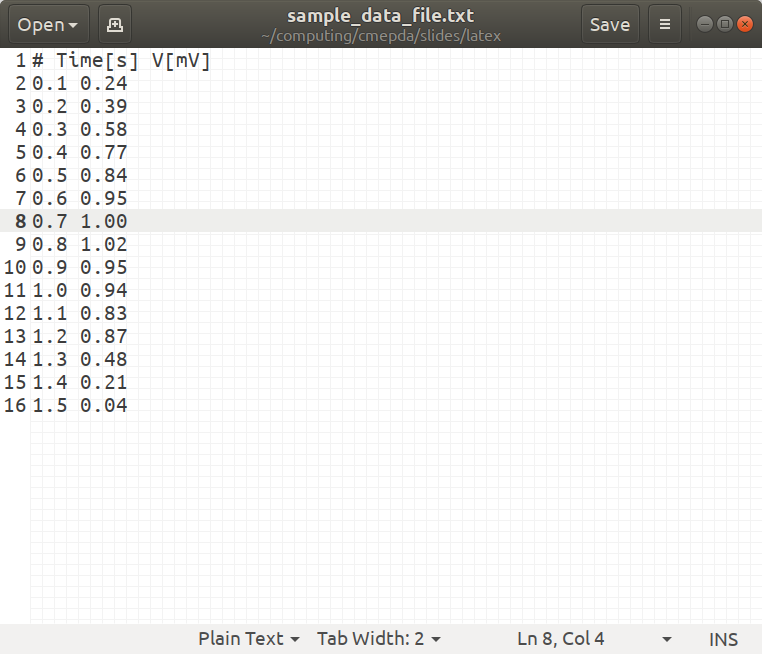
\includegraphics[width=0.8\textwidth]{voltage_file.png}
\end{frame}


\begin{frame}
  \frametitle{Solution - part 1}
  \begin{Verbatim}[label=\makebox{\url{https://github.com/lucabaldini/cmepda/tree/master/slides/latex/snippets/voltage\_data\_1.py}},commandchars=\\\{\}]
\PY{k+kn}{import} \PY{n+nn}{numpy}

\PY{k}{class} \PY{n+nc}{VoltageData}\PY{p}{:}
   \PY{l+s+sd}{\PYZdq{}\PYZdq{}\PYZdq{}Class for handling a set of measurements of the voltage at different}
\PY{l+s+sd}{   times.\PYZdq{}\PYZdq{}\PYZdq{}}
   
   \PY{k}{def} \PY{n+nf+fm}{\PYZus{}\PYZus{}init\PYZus{}\PYZus{}}\PY{p}{(}\PY{n+nb+bp}{self}\PY{p}{,}  \PY{n}{times}\PY{p}{,} \PY{n}{voltages}\PY{p}{)}\PY{p}{:}
       \PY{l+s+sd}{\PYZdq{}\PYZdq{}\PYZdq{} Constructor from two iterables (times and voltages)\PYZdq{}\PYZdq{}\PYZdq{}}
       \PY{n}{t} \PY{o}{=} \PY{n}{numpy}\PY{o}{.}\PY{n}{array}\PY{p}{(}\PY{n}{times}\PY{p}{,} \PY{n}{dtype}\PY{o}{=}\PY{n}{numpy}\PY{o}{.}\PY{n}{float}\PY{p}{)}
       \PY{n}{v} \PY{o}{=} \PY{n}{numpy}\PY{o}{.}\PY{n}{array}\PY{p}{(}\PY{n}{voltages}\PY{p}{,} \PY{n}{dtype}\PY{o}{=}\PY{n}{numpy}\PY{o}{.}\PY{n}{float}\PY{p}{)}
       \PY{c+c1}{\PYZsh{} Put together the arrays in a single matrix with column\PYZus{}stack }
       \PY{n+nb+bp}{self}\PY{o}{.}\PY{n}{\PYZus{}data} \PY{o}{=} \PY{n}{numpy}\PY{o}{.}\PY{n}{column\PYZus{}stack}\PY{p}{(}\PY{p}{(}\PY{n}{t}\PY{p}{,}\PY{n}{v}\PY{p}{)}\PY{p}{)}
   
   \PY{n+nd}{@classmethod}
   \PY{k}{def} \PY{n+nf}{from\PYZus{}file}\PY{p}{(}\PY{n+nb+bp}{cls}\PY{p}{,} \PY{n}{file\PYZus{}path}\PY{p}{)}\PY{p}{:}
       \PY{l+s+sd}{\PYZdq{}\PYZdq{}\PYZdq{} Alternate constructor from a data file, exploiting load\PYZus{}txt()\PYZdq{}\PYZdq{}\PYZdq{}}
       \PY{n}{t}\PY{p}{,} \PY{n}{v} \PY{o}{=} \PY{n}{numpy}\PY{o}{.}\PY{n}{loadtxt}\PY{p}{(}\PY{n}{file\PYZus{}path}\PY{p}{,} \PY{n}{unpack}\PY{o}{=}\PY{n+nb+bp}{True}\PY{p}{)}
       \PY{k}{return} \PY{n+nb+bp}{cls}\PY{p}{(}\PY{n}{t}\PY{p}{,} \PY{n}{v}\PY{p}{)}   
   
   \PY{n+nd}{@property}
   \PY{k}{def} \PY{n+nf}{timestamps}\PY{p}{(}\PY{n+nb+bp}{self}\PY{p}{)}\PY{p}{:}
       \PY{c+c1}{\PYZsh{} Use the slice syntax to select the first column}
       \PY{k}{return} \PY{n+nb+bp}{self}\PY{o}{.}\PY{n}{\PYZus{}data}\PY{p}{[}\PY{p}{:}\PY{p}{,} \PY{l+m+mi}{0}\PY{p}{]}
   
   \PY{n+nd}{@property}
   \PY{k}{def} \PY{n+nf}{voltages}\PY{p}{(}\PY{n+nb+bp}{self}\PY{p}{)}\PY{p}{:}
       \PY{c+c1}{\PYZsh{} Use the slice syntax to select the second column}
       \PY{k}{return} \PY{n+nb+bp}{self}\PY{o}{.}\PY{n}{\PYZus{}data}\PY{p}{[}\PY{p}{:}\PY{p}{,} \PY{l+m+mi}{1}\PY{p}{]}
\end{Verbatim}
\end{frame}


\begin{frame}
  \frametitle{Solution - part 2}
  \begin{Verbatim}[label=\makebox{\url{https://github.com/lucabaldini/cmepda/tree/master/slides/latex/snippets/voltage\_data\_2.py}},commandchars=\\\{\}]
\PY{k}{class} \PY{n+nc}{VoltageData}\PY{p}{:}

   \PY{l+s+sd}{\PYZdq{}\PYZdq{}\PYZdq{} Other methods here...\PYZdq{}\PYZdq{}\PYZdq{}}
   
   \PY{k}{def} \PY{n+nf+fm}{\PYZus{}\PYZus{}len\PYZus{}\PYZus{}}\PY{p}{(}\PY{n+nb+bp}{self}\PY{p}{)}\PY{p}{:}
       \PY{l+s+sd}{\PYZdq{}\PYZdq{}\PYZdq{} Number of data points (or columns in the file, which is the same) \PYZdq{}\PYZdq{}\PYZdq{}}
       \PY{k}{return} \PY{n+nb+bp}{self}\PY{o}{.}\PY{n}{\PYZus{}data}\PY{o}{.}\PY{n}{shape}\PY{p}{[}\PY{l+m+mi}{0}\PY{p}{]}
   
   \PY{k}{def} \PY{n+nf+fm}{\PYZus{}\PYZus{}getitem\PYZus{}\PYZus{}}\PY{p}{(}\PY{n+nb+bp}{self}\PY{p}{,} \PY{n}{index}\PY{p}{)}\PY{p}{:}
       \PY{c+c1}{\PYZsh{} We use composition and simply call \PYZus{}\PYZus{}getitem\PYZus{}\PYZus{} from \PYZus{}data}
       \PY{k}{return} \PY{n+nb+bp}{self}\PY{o}{.}\PY{n}{\PYZus{}data}\PY{p}{[}\PY{n}{index}\PY{p}{]}
   
   \PY{k}{def} \PY{n+nf+fm}{\PYZus{}\PYZus{}iter\PYZus{}\PYZus{}}\PY{p}{(}\PY{n+nb+bp}{self}\PY{p}{)}\PY{p}{:}
       \PY{l+s+sd}{\PYZdq{}\PYZdq{}\PYZdq{}Return the values row by row\PYZdq{}\PYZdq{}\PYZdq{}}
       \PY{c+c1}{\PYZsh{} We use a generator expression here. The syntax is very readible!}
       \PY{k}{for} \PY{n}{i} \PY{o+ow}{in} \PY{n+nb}{range}\PY{p}{(}\PY{n+nb}{len}\PY{p}{(}\PY{n+nb+bp}{self}\PY{p}{)}\PY{p}{)}\PY{p}{:}
           \PY{k}{yield} \PY{n+nb+bp}{self}\PY{o}{.}\PY{n}{\PYZus{}data}\PY{p}{[}\PY{n}{i}\PY{p}{,} \PY{p}{:}\PY{p}{]} 
           
   \PY{k}{def} \PY{n+nf+fm}{\PYZus{}\PYZus{}repr\PYZus{}\PYZus{}}\PY{p}{(}\PY{n+nb+bp}{self}\PY{p}{)}\PY{p}{:}
       \PY{l+s+sd}{\PYZdq{}\PYZdq{}\PYZdq{} Print the full content row by row \PYZdq{}\PYZdq{}\PYZdq{}}
       \PY{k}{return} \PY{l+s+s1}{\PYZsq{}}\PY{l+s+se}{\PYZbs{}n}\PY{l+s+s1}{\PYZsq{}}\PY{o}{.}\PY{n}{join}\PY{p}{(}\PY{l+s+s1}{\PYZsq{}}\PY{l+s+s1}{\PYZob{}\PYZcb{} \PYZob{}\PYZcb{}}\PY{l+s+s1}{\PYZsq{}}\PY{o}{.}\PY{n}{format}\PY{p}{(}\PY{n}{row}\PY{p}{[}\PY{l+m+mi}{0}\PY{p}{]}\PY{p}{,} \PY{n}{row}\PY{p}{[}\PY{l+m+mi}{1}\PY{p}{]}\PY{p}{)} \PY{k}{for} \PY{n}{row} \PY{o+ow}{in} \PY{n+nb+bp}{self}\PY{p}{)}
   
   \PY{k}{def} \PY{n+nf+fm}{\PYZus{}\PYZus{}str\PYZus{}\PYZus{}}\PY{p}{(}\PY{n+nb+bp}{self}\PY{p}{)}\PY{p}{:}
       \PY{l+s+sd}{\PYZdq{}\PYZdq{}\PYZdq{} Print the full content row\PYZhy{}by\PYZhy{}row with a nice formatting\PYZdq{}\PYZdq{}\PYZdq{}}
       \PY{n}{row\PYZus{}fmt} \PY{o}{=} \PY{l+s+s1}{\PYZsq{}}\PY{l+s+s1}{Row \PYZob{}\PYZcb{} \PYZhy{}\PYZgt{} \PYZob{}:.3f\PYZcb{} s, \PYZob{}:.1f\PYZcb{} mV}\PY{l+s+s1}{\PYZsq{}}
       \PY{n}{row\PYZus{}str\PYZus{}gen} \PY{o}{=} \PYZbs{}
               \PY{p}{(}\PY{n}{row\PYZus{}fmt}\PY{o}{.}\PY{n}{format}\PY{p}{(}\PY{n}{i}\PY{p}{,} \PY{n}{row}\PY{p}{[}\PY{l+m+mi}{0}\PY{p}{]}\PY{p}{,} \PY{n}{row}\PY{p}{[}\PY{l+m+mi}{1}\PY{p}{]}\PY{p}{)} \PY{k}{for} \PY{n}{i}\PY{p}{,} \PY{n}{row} \PY{o+ow}{in} \PY{n+nb}{enumerate}\PY{p}{(}\PY{n+nb+bp}{self}\PY{p}{)}\PY{p}{)}
       \PY{k}{return} \PY{l+s+s1}{\PYZsq{}}\PY{l+s+se}{\PYZbs{}n}\PY{l+s+s1}{\PYZsq{}}\PY{o}{.}\PY{n}{join}\PY{p}{(}\PY{n}{row\PYZus{}str\PYZus{}gen}\PY{p}{)}
\end{Verbatim}
\end{frame}


\begin{frame}
  \frametitle{Solution - part 3}
  \begin{Verbatim}[label=\makebox{\url{https://github.com/lucabaldini/cmepda/tree/master/slides/latex/snippets/voltage\_data\_3.py}},commandchars=\\\{\}]
\PY{k}{class} \PY{n+nc}{VoltageData}\PY{p}{:}

    \PY{l+s+sd}{\PYZdq{}\PYZdq{}\PYZdq{}Other methods here...\PYZdq{}\PYZdq{}\PYZdq{}}

    \PY{k}{def} \PY{n+nf}{plot}\PY{p}{(}\PY{n+nb+bp}{self}\PY{p}{,} \PY{n}{ax}\PY{o}{=}\PY{n+nb+bp}{None}\PY{p}{,} \PY{n}{fmt}\PY{o}{=}\PY{l+s+s1}{\PYZsq{}}\PY{l+s+s1}{bo}\PY{l+s+s1}{\PYZsq{}}\PY{p}{)}\PY{p}{:}
        \PY{l+s+sd}{\PYZdq{}\PYZdq{}\PYZdq{} Draw the data points.\PYZdq{}\PYZdq{}\PYZdq{}}
        \PY{k+kn}{from} \PY{n+nn}{matplotlib} \PY{k+kn}{import} \PY{n}{pyplot} \PY{k}{as} \PY{n}{plt}
        \PY{c+c1}{\PYZsh{} The user can provide an existing figure to add the plot, otherwise we}
        \PY{c+c1}{\PYZsh{} create a new one.}
        \PY{k}{if} \PY{n}{ax} \PY{o+ow}{is} \PY{o+ow}{not} \PY{n+nb+bp}{None}\PY{p}{:}
            \PY{n}{plt}\PY{o}{.}\PY{n}{sca}\PY{p}{(}\PY{n}{ax}\PY{p}{)} \PY{c+c1}{\PYZsh{} sca (Set Current Axes) selects the given figure}
        \PY{k}{else}\PY{p}{:}
            \PY{n}{ax} \PY{o}{=} \PY{n}{plt}\PY{o}{.}\PY{n}{figure}\PY{p}{(}\PY{l+s+s1}{\PYZsq{}}\PY{l+s+s1}{voltage\PYZus{}vs\PYZus{}time}\PY{l+s+s1}{\PYZsq{}}\PY{p}{)}
        \PY{n}{plt}\PY{o}{.}\PY{n}{plot}\PY{p}{(}\PY{n+nb+bp}{self}\PY{o}{.}\PY{n}{timestamps}\PY{p}{,} \PY{n+nb+bp}{self}\PY{o}{.}\PY{n}{voltages}\PY{p}{,} \PY{n}{fmt}\PY{p}{)}
        \PY{n}{plt}\PY{o}{.}\PY{n}{xlabel}\PY{p}{(}\PY{l+s+s1}{\PYZsq{}}\PY{l+s+s1}{Time [s]}\PY{l+s+s1}{\PYZsq{}}\PY{p}{)}
        \PY{n}{plt}\PY{o}{.}\PY{n}{ylabel}\PY{p}{(}\PY{l+s+s1}{\PYZsq{}}\PY{l+s+s1}{Voltage [mV]}\PY{l+s+s1}{\PYZsq{}}\PY{p}{)}
        \PY{n}{plt}\PY{o}{.}\PY{n}{grid}\PY{p}{(}\PY{n+nb+bp}{True}\PY{p}{)}
        \PY{k}{return} \PY{n}{ax} \PY{c+c1}{\PYZsh{} We return the axes, just in case }
\end{Verbatim}
\end{frame}


\begin{frame}
  \frametitle{Output plot}
  \centering
  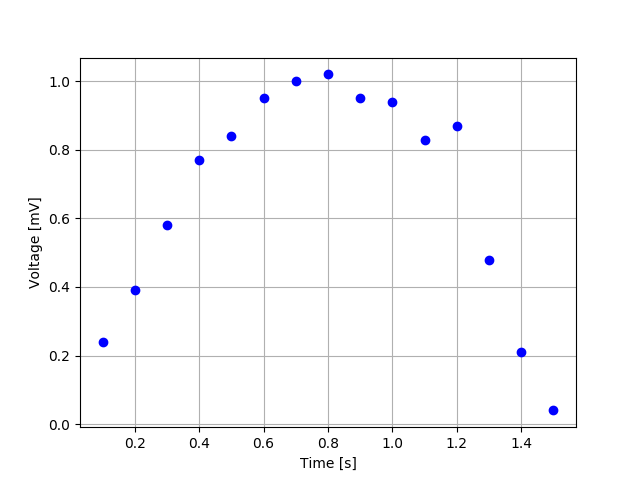
\includegraphics[width=0.8\textwidth]{voltage_vs_time.png}
\end{frame}


\begin{frame}
  \frametitle{Put yourself to test}
  \begin{itemize}
    \item Manage a third column - optional - with voltage errors
    \item Write a proper unittest module for the class
    \item The full current version of the class is in snippets/voltage\_data.py
  \end{itemize}  
  
\end{frame}


%\begin{frame}
%  \frametitle{Why is that useful?}
%  \framesubtitle{A real life example}
%  \begin{itemize}
%    \item Suppose you have an image where each pixel is represented by a pair
%          of coordinates and a value z (like the charge from a pixel imaging detector)
%    \item You want to rotate each image so that the x-axis is the principal 
%          axis of the inertia ellipsoid of the 2-D distribution of z
%    \item For each image you need first to calculate the direction of the principal
%          axis, then rotate the coordinates of each pixel with the rotation matrix
%  \end{itemize}
%  
%  \[
%  M=
%    \begin{pmatrix}
%      \cos{(\theta)} & \sin{(\theta)} \\
%      - \sin{(\theta)} & \cos{(\theta)}
%    \end{pmatrix}
%  \]
%  
%  \begin{itemize}
%    \item Where $\theta$ is the angle between the principal axis and the x-axis
%    \item Ho do you write the rotation function?
%  \end{itemize}
% 
%\end{frame}


\end{document}
